\documentclass[a4paper,11pt,titlepage]{report}
\usepackage[utf8]{inputenc}   % permet l'utilisation de caractres ISO
\usepackage[french]{babel}    % choix du francais
\usepackage{fancyhdr}       % ncessaire pour \pagestyle{fancy}
\usepackage{fancybox}
\usepackage[dvips]{graphicx}       % gestion des images
\usepackage{placeins}   % gestion de la position des images
\usepackage{amsmath}        % modification des polices mathmatiques
\usepackage{amssymb}
\usepackage{mathrsfs}
\usepackage[cyr]{aeguill}
\usepackage{enumitem}
\usepackage{pifont}
\usepackage{psfrag}
\usepackage{epsfig}
\usepackage{supertabular}
\usepackage{array}
\usepackage{multicol}
\usepackage{multirow} % Pour faire des tableaux contenant des lignes fusionnes
\usepackage{hyperref}
\usepackage{color}
\usepackage[dvipsnames]{pstricks}
\usepackage{pstricks-add,pst-plot,pst-node}
\usepackage[dvipsnames]{xcolor}
\usepackage{enumerate}
\usepackage{float}
\usepackage{titlesec}
\usepackage{textcomp}
\usepackage{subfigure}
\usepackage{sectsty}
\usepackage{pdfpages}
\usepackage{etex} % permet de charger plus de package 
\usepackage{listings}

%===============================
% Mise en page chapitre ligne verticale TD
%------------------------------------------
\makeatletter
\def\thickhrulefill{\leavevmode \leaders \hrule height 1ex \hfill \kern \z@}
\def\@makechapterhead#1{%
  \vspace*{10\p@}%
  {\parindent \z@ 
        \raggedleft
        \reset@font\huge\bfseries
        \begin{tabular}{l|p{13cm}}
         \textcolor{rltred}{ { TD  }}
          &\
          \Huge #1
        \end{tabular}
        \par\nobreak
    \vskip 70\p@
  }}

%===============================
% Definition des couleurs 
%------------------------------------------
\definecolor{rltred}{rgb}{0.75,0,0}    
\definecolor{rltgreen}{rgb}{0,0.5,0}
\definecolor{oneblue}{rgb}{0,0,0.6}
\definecolor{marron}{rgb}{0.64,0.16,0.16}
\definecolor{forestgreen}{rgb}{0.13,0.54,0.13}
\definecolor{purple}{rgb}{0.62,0.12,0.94}
\definecolor{dockerblue}{rgb}{0.11,0.56,0.98}
\definecolor{freeblue}{rgb}{0.25,0.41,0.88}
\definecolor{freeblue2}{rgb}{0.25,0.41,0.77}
\definecolor{myblue}{rgb}{0,0.2,0.4}

%===============================
% Definition de l'affichage des sections et sous sections
%------------------------------------------
\renewcommand{\sectionmark}[1]{\markright{\thesection\ #1}}
\renewcommand{\headrulewidth}{0.4pt}   % trait horizontal en dessous de l'entete
\renewcommand{\footrulewidth}{0.4pt}     % trait horizontal au dessus du pied de page
\renewcommand{\baselinestretch}{1.1} % augmente l'interligne  1.1
    
\renewcommand{\thesection}{\Roman{section}}
\renewcommand{\thechapter}{\arabic{chapter}}

\usepackage{geometry}
\geometry{ hmargin=3cm, vmargin=2.5cm }
\headheight=15pt
\textwidth=170mm \oddsidemargin=-4mm %\evensidemargin=0mm

%% Profondeur de \subsubsection = 3
\setcounter{tocdepth}{2} % pour que les subsubsection apparaissent dans la table des matieres
\setcounter{secnumdepth}{3} % pour que les subsubsection soient numrotes

% Pouvoir afficher des URL correctement
\usepackage{url}
\let\urlorig\url
\renewcommand{\url}[1]{%
  \begin{otherlanguage}{english}\urlorig{#1}\end{otherlanguage}%
}


%===============================
% Définition de nouvelles commandes de listes
%------------------------------------------
\newlist{coche}{itemize}{2}
\setlist[coche, 1]{font=\color{rltred} , label=\ding{51}}
\setlist[coche, 2]{font=\color{rltred}}

\newlist{point}{itemize}{2}
\setlist[point, 1]{label=\textbullet}
\setlist[point, 2]{label=--}

\newlist{tiret}{itemize}{2}
\setlist[tiret, 1]{label=--}
\setlist[tiret, 2]{label=-}

%===============
% Environnements 
%--------------------
\newcommand{\Obj}[1]{\noindent
\rule[0.1cm]{1cm}{0.8pt} \textbf{Objectif} \rule[0.1cm]{14.1cm}{0.8pt}\\
#1\\
\rule[0.1cm]{17cm}{0.8pt} }

\newcommand{\Pbm}[1]{\noindent
\textcolor{rltred}{\rule[0.1cm]{1cm}{0.8pt}} \textbf{Problématique technique} \textcolor{rltred}{\rule[0.1cm]{11cm}{0.8pt}}\\
#1\\
\textcolor{rltred}{\rule[0.1cm]{17cm}{0.8pt}}}
   
\newcounter{Qu}
\addtocounter{Qu}{+1}
\newcommand{\Q}{\noindent \textbf{Q\theQu .\hspace{0,7mm}}\addtocounter{Qu}{+1}}

\newcounter{Exem}
\addtocounter{Exem}{+1}
% \newcommand{\Exem}{\noindent \textbf{Exemple: \hspace{0,7mm}}\addtocounter{Exem}{+1}}
\newcommand{\Exem}[1]{\noindent \fcolorbox{lightgray}{lightgray}{\begin{minipage}[c]{16.7cm}\textbf{Exemple\hspace{0,8mm} \theExem \hspace{0,8mm}}\addtocounter{Exem}{+1}:  \textit{#1}\end{minipage}}}


\newcounter{Ex}
\addtocounter{Ex}{+1}
\newcommand{\E}{\noindent \textbf{Ex\theEx .\hspace{0,7mm}}\addtocounter{Ex}{+1}}

\newcounter{Prop}
\addtocounter{Prop}{+1}
\newcommand{\Prop}[1]{\noindent \fcolorbox{lightgray}{lightgray}{\begin{minipage}[c]{16.7cm}\textbf{Propriété\hspace{0,8mm} \theProp \hspace{0,8mm}}\addtocounter{Prop}{+1} \textit{#1}\end{minipage}}}

\newcounter{Def}
\addtocounter{Def}{+1}
\newcommand{\Def}[1]{\noindent \fcolorbox{lightgray}{lightgray}{\begin{minipage}[c]{16.75cm}\textbf{Définition\hspace{0,8mm} \theDef \hspace{0,8mm}}\addtocounter{Def}{+1} \textit{#1}\end{minipage}}}

\newcounter{Thm}
\addtocounter{Thm}{+1}
\newcommand{\Thm}[1]{\noindent \fcolorbox{lightgray}{lightgray}{\begin{minipage}[c]{16.7cm}\textbf{Théorème\hspace{0,8mm} \theThm \hspace{0,8mm}}\addtocounter{Thm}{+1} \textit{#1}\end{minipage}}}

\newcommand{\Man}[1]{\noindent
\textcolor{blue}{\rule[0.1cm]{1cm}{0.8pt}} \textcolor{blue}{\textbf{Manipulation}} \textcolor{blue}{\rule[0.1cm]{13.2cm}{0.8pt}}\\ \textcolor{blue}{#1}\\
\textcolor{blue}{\rule[0.1cm]{17cm}{0.8pt}}}


\definecolor{gris25}{gray}{0.75}
\definecolor{bleu}{RGB}{18,33,98}
\definecolor{bleuf}{RGB}{42,94,171}
\definecolor{bleuc}{RGB}{231,239,247}
\definecolor{rougef}{RGB}{185,18,27}
\definecolor{rougec}{RGB}{255,230,231}
\definecolor{vertf}{RGB}{103,126,82}
\definecolor{vertc}{RGB}{220,255,191}
\definecolor{violetf}{RGB}{112,48,160}
\definecolor{violetc}{RGB}{230,224,236}
%

\newenvironment{py}[1][\hsize]%
{%
    \def\FrameCommand%
    {%
%\rotatebox{90}{\textit{\textsf{Python}}} 
\rotatebox{90}{
\includegraphics[height=.6cm]{../images/logo_python}} 
        {\color{violetf}\vrule width 3pt}%
        \hspace{0pt}%must no space.
        \fboxsep=\FrameSep\colorbox{violetc}%
    }%
    \MakeFramed{\hsize #1 \advance\hsize-\width\FrameRestore}%
}%
{\endMakeFramed}%


%  Code python
%%%%%%%%%%%%%%%%%%%%%%%%%%%%

\definecolor{fond}{rgb}{1,1,1}			%Couleur du fond
\definecolor{commentaires}{rgb}{0.5,0.5,0.5}	%Couleur des commentaires
\definecolor{chaines}{rgb}{0,0.63,0}		%Couleur des chaines de caracteres
\definecolor{fonctions}{rgb}{0,0,1}		%Couleur des fonctions de bases
\definecolor{decoration}{rgb}{0.5,0.5,0.5}		%Couleur des fonctions autre (??)
\definecolor{self}{rgb}{0,0,0}		%je sais pas. J'ai recopié d'internet
\definecolor{numeros}{rgb}{0.7,0.7,0.7}		%numéros de ligne
\definecolor{chevrons}{rgb}{1,0.,0.}		%chevrons


\lstset{
	%Langage
		language=Python,	%Langage par défaut
	%Mise en forme de l'environnement
		xleftmargin=2em,	%marge a gauche
		%frame=trBL,		%Cadre (double cadre)
		backgroundcolor=\color{fond},	%Couleur d'arriere plan
		framexleftmargin=5mm,
		frame=shadowbox,
		rulesepcolor=\color{black},
		texcl=true,	%Activle les commandes LaTex dans le code
		%escapechar=ø,	%Caractere a echapper
		escapeinside={(*}{*)},
	%Numeros de ligne
		numbers=left,	%Rajoute des numéros de ligne
		numberstyle=\footnotesize\color{numeros},	%Taille des numéros de ligne
		numbersep=1em,			%Marge entre le code et les numéros de ligne
	%Mise en forme du texte
		columns=fixed,		%Largeur des lettres (fixed, flexible, fullflexible)
		basicstyle=\ttfamily,	%Mise en forme de base
		showspaces=false,	%Pour mettre des especes d'underscore sur les espaces
		tabsize=8,	%Taille des tabulations	
	%Commentaires
		commentstyle=\color{commentaires}\slshape,	%Couleur des commentaires
	%Chaine de caracteres
		stringstyle=\color{chaines},
		showstringspaces=false,
		morecomment=[s][\color{chaines}]{"""}{"""},
		morecomment=[s][\color{chaines}]{'''}{'''},
	%Fonctions et mot clé de python
		morekeywords={import,from,class,def,for,while,if,is,in,elif,else,not,and,or,print,break,continue,return,True,False,None,access,as,del,except,exec,finally,global,import,lambda,pass,print,raise,try,assert},
		keywordstyle=\color{fonctions}\bfseries,
		morekeywords={[3]>>>},
		keywordstyle={[3]\color{chevrons}\bfseries},
		morekeywords={[2]@invariant},
		keywordstyle={[2]\color{decoration}\slshape},
		emph={self},
		emphstyle={\color{self}\slshape}
	}
\lstnewenvironment{codePython}
		{	\footnotesize\setbox1=\vbox
			\bgroup
		}
		{	\egroup	
			\begin{center}
				\begin{minipage}{0.8\linewidth}
					%\begin{bclogo}[couleur=white,logo=\bcoutil,noborder = true]{Code Python}
						\box1
					%\end{bclogo}
				\end{minipage}
			\end{center}
		}

%%%%%%%%%%%%%%%%%%%%%%%%%%%%%%%%%%%%%%%%%%
% PseudoCode
%%%%%%%%%%%%%%%%%%%%%%%%%%%%%%%%%%%%%%%%%%

\definecolor{fond_pseudo}{RGB}{250,250,250} %Couleur du fond
\definecolor{bord_pseudo}{RGB}{0,0,0} %Couleur du fond

\newcounter{cptPseudo}

\newenvironment{pseudoCode}[1][]	{\refstepcounter{cptPseudo}
				\begin{center}
					\begin{minipage}{0.95\linewidth}
						\begin{bclogo}[couleur=fond_pseudo,couleurBord=bord_exemple,arrondi=0.2,logo=\bcbook]{pseudo code \ : \emph{#1}}}
				{		\end{bclogo}
					\end{minipage}
				\end{center}}		
		
		
% \lstnewenvironment{codepseudo}
% 		{	\footnotesize\setbox1=\vbox
% 			\bgroup
% 		}
% 		{	\egroup	
% 			\begin{center}
% 			\begin{minipage}{0.05\linewidth}
% 			 {
\includegraphics[angle=90,width=0.45\linewidth]{../image/pseudo_code_image.png}}
% 			\end{minipage}\begin{minipage}{0.7\linewidth}
% 					%\begin{bclogo}[couleur=white,logo=\bcoutil,noborder = true]{Code Python}
% 						\box1
% 					%\end{bclogo}
% 				\end{minipage}
% 			\end{center}
% 		}		
\lstnewenvironment{codePseudo}
		{	\footnotesize\setbox1=\vbox
			\bgroup
		}
		{	\egroup	
			\begin{center}
				\begin{minipage}{0.8\linewidth}
					%\begin{bclogo}[couleur=white,logo=\bcoutil,noborder = true]{Code Python}
						\box1
					%\end{bclogo}
				\end{minipage}
			\end{center}
		}
		
		
		
		
		
		
\lstnewenvironment{pseudo}[1][]{
% 		\rotatebox{90}{\textit{\textsf{Pseudo Code}}} 
\lstset{
language=pseudocode,
basicstyle=\sffamily\footnotesize, 	
stringstyle=\color{red}, 
showstringspaces=false, 
alsoletter={1234567890},
otherkeywords={\ , \}, \{},
keywordstyle=\color{blue},
emph={pour, faire, varie, si, tant que, et, ou, Fonction, alors, sinon, fin si},
emphstyle=\color{black}\bfseries,
emph={[2]True, False, None, self},
emphstyle=[2]\color{olive},
emph={[3]from, import, as},
emphstyle=[3]\color{blue},
upquote=true,
columns=flexible, % pour empecher d'avoir un espacement mono
morecomment=[s]{"""}{"""},
commentstyle=\color{Hellbraun}\backslash\backslash,
%emph={[4]1, 2, 3, 4, 5, 6, 7, 8, 9, 0},
emphstyle=[4]\color{blue},
literate=*{:}{{\textcolor{blue}:}}{1}
{=}{{\textcolor{blue}=}}{1}
{-}{{\textcolor{blue}-}}{1}
{+}{{\textcolor{blue}+}}{1}
{*}{{\textcolor{blue}*}}{1}
{!}{{\textcolor{blue}!}}{1}
{(}{{\textcolor{blue}(}}{1}
{)}{{\textcolor{blue})}}{1}
{[}{{\textcolor{blue}[}}{1}
{]}{{\textcolor{blue}]}}{1}
{<}{{\textcolor{blue}<}}{1}
{>}{{\textcolor{blue}>}}{1},
%framexleftmargin=1mm, framextopmargin=1mm, frame=shadowbox, rulesepcolor=\color{blue},#1
%backgroundcolor=\color{SourceHintergrund}, 
%framexleftmargin=1mm, framexrightmargin=1mm, framextopmargin=1mm, frame=single, framerule=1pt, rulecolor=\color{black},#1
}}{}

				
\NeedsTeXFormat{LaTeX2e}[1999/01/01]
\ProvidesPackage{schemabloc}[2006/12/29]

\RequirePackage{ifthen}
\RequirePackage{tikz}
\usetikzlibrary{shapes,arrows}


%macros dessin des sch�ma-blocs mise � jour 6 janvier 2009
% version 1.5

%initialisation des styles
\tikzstyle{sbStyleLien}=[->,>=latex',]
\tikzstyle{sbStyleBloc}=[draw, rectangle,]
\tikzstyle{sbStyleBlocPatate}=[]
\tikzstyle{sbStyleSum}=[draw, circle,]%style Sum CC
% Commandes de changement de style
\newcommand{\sbStyleLienDefaut}{
\tikzstyle{sbStyleLien}=[->,>=latex']
}

\newcommand{\sbStyleLien}[1]{
\tikzstyle{sbStyleLien}+=[#1]
}

\newcommand{\sbStyleBloc}[1]{
\tikzstyle{sbStyleBloc}+=[#1]
}
\newcommand{\sbStyleBlocDefaut}{
\tikzstyle{sbStyleBloc}=[draw, rectangle,]
}

\newcommand{\sbStyleSum}[1]{
\tikzstyle{sbStyleSum}+=[#1]
}

\newcommand{\sbStyleSumDefaut}{
\tikzstyle{sbStyleBloc}=[draw, circle,]
}%style Sum default CC


% Commandes d'entr�e et sortie
\newcommand{\sbEntree}[1]{
    \node [coordinate, name=#1] {};
\sbDecaleNoeudx[0]{#1}{#1}
}
\newcommand{\sbSortie}[3][2]{
    \node [coordinate, right of=#3droite, node distance=#1em, minimum size=0em,right] (#2) {};
}

%Commandes de Bloc
\newcommand{\sbBloc}[4][2]{
\node [draw, rectangle, 
    minimum height=3em, minimum width=3em, right of = #4droite,
node distance=#1em,sbStyleBloc,right] (#2) {#3};
\node (#2droite) at (#2.east){};
\node (BlocdeFindroite) at (#2.east){};
}

\newcommand{\sbBlocPatate}[4][2]{
\node [draw, cloud, cloud puffs=5, draw, 
    minimum height=3em, minimum width=5em, right of = #4droite,
node distance=#1em,sbStyleBlocPatate,right] (#2) {#3};
\node (#2droite) at (#2.east){};
}

\newcommand{\sbBlocr}[4][2]{
\node [ 
    minimum height=3em, minimum width=3em, left of = #4gauche, 
node distance=#1em, sbStyleBloc,left] (#2) {#3};
\node (#2gauche) at (#2.west){};
}

\newcommand{\sbBlocL}[4][2]{
\node [draw, rectangle, 
    minimum height=3em, minimum width=3em, right of = #4droite,node distance=#1em,sbStyleBloc,right] (#2) {#3};
\node (#2droite) at (#2.east){};
\node (BlocdeFindroite) at (#2.east){};
 \draw [sbStyleLien,auto] (#4) -- node[name=#4-#2] {} (#2);
}

\newcommand{\sbBlocrL}[4][2]{
\node [draw, rectangle, 
    minimum height=3em, minimum width=3em, left of = #4gauche, 
node distance=#1em, sbStyleBloc,left] (#2) {#3};
\node (#2gauche) at (#2.west){};
\node (BlocdeFingauche) at (#2.west){};
 \draw [sbStyleLien,auto] (#4) -- node[name=#4-#2] {} (#2);
}

\newcommand{\sbBlocseul}[4][1.5]{
\sbEntree{E1}
\sbBloc[#1]{B1}{#3}{E1}
\sbSortie[#1]{S1}{B1}
\sbRelier{E1}{B1}{#2}
\sbRelier{B1}{S1}{#4}
}

%\Commande de lien
\newcommand{\sbRelier}[3][]{
 \draw [sbStyleLien,auto] (#2) -- node[name=#2-#3] {#1} (#3);
}

\newcommand{\sbRelieryx}[2]{
\draw [sbStyleLien] (#1.south)  |-   (#2)  ;
}
\newcommand{\sbRelierxy}[3][]{
\draw [sbStyleLien] (#2)  -|   node[name=#2-#3,near end,right] {#1} (#3) ;
}

\newcommand{\sbRenvoi}[4][4]{
\node [below of=#2, node distance=#1em, minimum size=0em](retour#2) {};
\draw [sbStyleLien] (#2.south)--(retour#2.south)   -|   node[name=#2-#3,near end,right] {#4} (#3) ;
}

\newcommand{\sbNomLien}[3][0.4]{
\node[above of=#2, node distance=#1em] (#2nom) at (#2) {#3};
}
%Commande comparateurs et sommateurs

\newcommand*{\sbCompSum}{\@ifstar\sbCompSumNorm\sbCompSumUsuel}

\newcommand{\sbCompSumUsuel}[7][4]{
    \node [draw, circle,minimum size=2em, right of=#3,node distance=#1em] (#2) {};
	 \node [draw, cross out,minimum size=1.414em,right of=#3,node distance=#1em] {};
	 \node [above of=#2,node distance=0.6em] {$#4$};
	 \node [below of=#2,node distance=0.6em] {$#5$};
	 \node [left of=#2,node distance=0.6em] {$#6$};
	 \node [right of=#2,node distance=0.6em] {$#7$};
\node (#2droite) at (#2.east){};
\node (#2gauche) at (#2.west){};
}

\newcommand{\sbCompSumNorm}[7][4]{
    \node [draw, circle,minimum size=1.5em, right of=#3,node distance=#1em,
label=85:$#4$,label=-85:$#5$,label=175:$#6$,label=5:$#7$,sbStyleSum] (#2) {};
\node (#2droite) at (#2.east){};
\node (#2gauche) at (#2.west){};
}

\newcommand{\sbSum}[6][4]{
    \node [draw, circle,minimum size=1.5em, right of=#3,node distance=#1em,
label=175:$#4$,label=-85:$#5$,label=85:$#6$,sbStyleSum] (#2) {};
\node (#2droite) at (#2.east){};
\node (#2gauche) at (#2.west){};
}

\newcommand*{\sbComp}{\@ifstar\sbCompNorm\sbCompUsuel}
\newcommand{\sbCompUsuel}[3][4]{
\sbCompSum[#1]{#2}{#3}{}{-}{+}{}
}
\newcommand{\sbCompNorm}[3][4]{
\sbCompSum*[#1]{#2}{#3}{}{-}{+}{}
}


\newcommand*{\sbComph}{\@ifstar\sbComphNorm\sbComphUsuel}
\newcommand{\sbComphUsuel}[3][4]{
\sbCompSum[#1]{#2}{#3}{-}{}{+}{}
}

\newcommand{\sbComphNorm}[3][4]{
\sbCompSum*[#1]{#2}{#3}{-}{}{+}{}
}

\newcommand*{\sbSumh}{\@ifstar\sbSumhNorm\sbSumhUsuel}
\newcommand{\sbSumhUsuel}[3][4]{
\sbCompSum[#1]{#2}{#3}{+}{}{+}{}
}
\newcommand{\sbSumhNorm}[3][4]{
\sbCompSum*[#1]{#2}{#3}{+}{}{+}{}
}

\newcommand*{\sbSumb}{\@ifstar\sbSumbNorm\sbSumbUsuel}
\newcommand{\sbSumbUsuel}[3][4]{
\sbCompSum[#1]{#2}{#3}{}{+}{+}{}
}
\newcommand{\sbSumbNorm}[3][4]{
\sbCompSum*[#1]{#2}{#3}{}{+}{+}{}
}


%Commandes de d�calage de noeud

\newcommand{\sbDecaleNoeudy}[3][5]{
\node [below of=#2, node distance=#1em, minimum size=0em](#3) {};
\node (#3droite) at (#3){};
\node (#3gauche) at (#3){};
}
\newcommand{\sbDecaleNoeudx}[3][5]{
\node [right of=#2, node distance=#1em, minimum size=0em](#3) {};
\node (#3droite) at (#3){};
\node (#3gauche) at (#3){};
}


%==============Chaines et Boucles===========

\newcommand{\sbChaine}[3][4]{
\foreach \x/\y [remember=\x as \lastx (initially #2)] in {#3}
{\sbBlocL[#1]{\x}{\y}{\lastx}
}
}

\newcommand{\sbChaineRetour}[3][4]{
\foreach \x/\y [remember=\x as \lastx (initially #2)] in {#3}
{\sbBlocrL[#1]{\x}{\y}{\lastx}
}
}

\newcommand{\sbBoucleSeule}[4][4]{
\sbComp[#1]{Comp#2}{#2}\sbRelier{#2}{Comp#2}
\sbChaine[#1]{Comp#2}{#3}
\sbSortie[#1]{#4}{BlocdeFin}
\draw [sbStyleLien,auto] (BlocdeFindroite.base) -- node[name=FindeChaine-#4] {} (#4);
\sbRenvoi{FindeChaine-#4}{Comp#2}{}
}


\newcommand{\sbBoucle}[3][4]{
\sbComp[#1]{Comp#2}{#2}\sbRelier{#2}{Comp#2}
\sbChaine[#1]{Comp#2}{#3}
\draw [sbStyleLien,auto,-] (BlocdeFindroite.base) --++(1em,0)coordinate[name=FindeChaine];
\sbRenvoi{FindeChaine}{Comp#2}{}
}

\newcommand{\sbBoucleRetour}[4][4]{
\sbComp[#1]{Comp#2}{#2}\sbRelier{#2}{Comp#2}
\sbChaine[#1]{Comp#2}{#3}
\draw [sbStyleLien,auto,-] (BlocdeFindroite.base) --++(1em,0)coordinate[name=FindeChaine];
\sbDecaleNoeudy[5]{FindeChaine}{sbDebutRetour}
\sbChaineRetour[#1]{sbDebutRetour}{#4}
\draw [sbStyleLien,-] (FindeChaine)  |-   (sbDebutRetour.west)  ;

\draw [sbStyleLien] (BlocdeFingauche.base)  -|   node[name=sbNomRetour,near end,right] {} (Comp#2) ;

}




%vielles definitions, ne plus utiliser, d�commenter si n�cessaire
%\newcommand{\bloc}[4][2]{
%\node [draw, rectangle, 
%    minimum height=1cm, minimum width=1cm, right of = #4,node distance=#1cm] (#2) {#3};
%}
%\newcommand{\blocr}[4][1.5]{
%\node [draw, rectangle, 
%    minimum height=1cm, minimum width=1cm, left of = #4, node distance=#1cm] (#2) {#3};
%}
%\newcommand{\comp}[3][1.5]{
%    \node [draw, circle,minimum size=1cm, right of=#3,node distance=#1cm] (#2) {};
%	 \node [draw, cross out,minimum size=0.707cm,right of=#3,node distance=#1cm] {};
%	 \node [below of=#2,node distance=0.3cm] {$-$};
%		\node [left of=#2,node distance=0.3cm] {$+$};
%}
%\newcommand{\comph}[3][2]{
%    \node [draw, circle,minimum size=1cm, right of=#3,node distance=#1cm] (#2) {};
%	 \node [draw, cross out,minimum size=0.707cm,right of=#3,node distance=#1cm] {};
%	 \node [above of=#2,node distance=0.3cm] {$-$};
%		\node [left of=#2,node distance=0.3cm] {$+$};
%}
%\newcommand{\sumh}[3][2]{
%    \node [draw, circle,minimum size=1cm, right of=#3,node distance=#1cm] (#2) {};
%	 \node [draw, cross out,minimum size=0.707cm,right of=#3,node distance=#1cm] {};
%	 \node [above of=#2,node distance=0.3cm] {$+$};
%		\node [left of=#2,node distance=0.3cm] {$+$};
%}
%\newcommand{\sumb}[3][2]{
%    \node [draw, circle,minimum size=1cm, right of=#3,node distance=#1cm] (#2) {};
%	 \node [draw, cross out,minimum size=0.707cm,right of=#3,node distance=#1cm] {};
%	 \node [below of=#2,node distance=0.3cm] {$+$};
%		\node [left of=#2,node distance=0.3cm] {$+$};
%}
%
%\newcommand{\entree}[1]{
%    \node [coordinate, name=#1,node distance=1cm] {};
%}
%\newcommand{\sortie}[3][1.5]{
%    \node [coordinate, right of=#3, node distance=#1cm, minimum size=0cm] (#2) {};
%}
%\newcommand{\decale}[3][2]{
%\node [below of=#2, node distance=#1cm, minimum size=0cm](#3) {};
%}
%
%\newcommand{\relier}[3]{
% \draw [->,>=latex',auto] (#1) -- node[name=#1-#2] {#3} (#2);
%}
%\newcommand{\relieryx}[2]{
%\draw [->,>=latex'] (#1.south)  |-   (#2)  ;
%}
%\newcommand{\relierxy}[3]{
%\draw [->,>=latex'] (#1)  -|   node[name=#1-#2,near end,right] {#3} (#2) ;
%}
%\newcommand{\renvoi}[4][1.5]{
%\node [below of=#2, node distance=#1cm, minimum size=0cm](retour#2) {};
%\draw [->,>=latex'] (#2.south)--(retour#2.south)   -|   node[name=#2-#3,near end,right] {#4} (#3) ;
%}
%\newcommand{\blocseul}[4][1.5]{
%\entree{E1}
%\bloc[#1]{B1}{#3}{E1}
%\sortie[#1]{S1}{B1}
%\relier{E1}{B1}{#2}
%\relier{B1}{S1}{#4}
%}


%configure hyperref
\hypersetup{
backref=true, %permet d'ajouter des liens dans...
pagebackref=true,%...les bibliographies
hyperindex=true, %ajoute des liens dans les index.
colorlinks=true, %colorise les liens
breaklinks=true, %permet le retour  la ligne dans les liens trop longs
urlcolor= black, %couleur des hyperliens
linkcolor= black, %couleur des liens internes
bookmarks=true, %cr des signets pour Acrobat
bookmarksopen=true, %si les signets Acrobat sont crs les afficher completement.
pdftitle={TP informatique}, %informations apparaissant
pdfauthor={upsti}, %dans les informations du document
pdfsubject={GT info} }%sous Acrobat.
% \newcommand	{\competences}		{\begin{itemize}
% \item A - compétences 1
% \end{itemize}	}    
%--------------------------------------------------------%
%--------------------------------------------------------%

\graphicspath{{image/}}
\newcommand	{\partie}		{TP5}
\newcommand  {\partiehaute}	{TP5}
\newcommand	{\titre}		{TP5 -- Bibliothèques, fichiers, graphiques}
\newcommand	{\numero}		{1}
\newcommand	{\type}		{TP}
\newcommand	{\version}		{V1}


% \documentclass[a4paper,11pt]{article}
% \usepackage[utf8]{inputenc}   % permet l'utilisation de caractres ISO
\usepackage[french]{babel}    % choix du francais
\usepackage{fancyhdr}       % ncessaire pour \pagestyle{fancy}
\usepackage{fancybox}
\usepackage[dvips]{graphicx}       % gestion des images
\usepackage{placeins}   % gestion de la position des images
\usepackage{amsmath}        % modification des polices mathmatiques
\usepackage{amssymb}
\usepackage{mathrsfs}
\usepackage[cyr]{aeguill}
\usepackage{enumitem}
\usepackage{pifont}
\usepackage{psfrag}
\usepackage{epsfig}
\usepackage{supertabular}
\usepackage{array}
\usepackage{multicol}
\usepackage{multirow} % Pour faire des tableaux contenant des lignes fusionnes
\usepackage{hyperref}
\usepackage{color}
\usepackage[dvipsnames]{pstricks}
\usepackage{pstricks-add,pst-plot,pst-node}
\usepackage[dvipsnames]{xcolor}
\usepackage{enumerate}
\usepackage{float}
\usepackage{titlesec}
\usepackage{textcomp}
\usepackage{subfigure}
\usepackage{sectsty}
\usepackage{pdfpages}
\usepackage{etex} % permet de charger plus de package 
\usepackage{listings}

%===============================
% Mise en page chapitre ligne verticale TD
%------------------------------------------
\makeatletter
\def\thickhrulefill{\leavevmode \leaders \hrule height 1ex \hfill \kern \z@}
\def\@makechapterhead#1{%
  \vspace*{10\p@}%
  {\parindent \z@ 
        \raggedleft
        \reset@font\huge\bfseries
        \begin{tabular}{l|p{13cm}}
         \textcolor{rltred}{ { TD  }}
          &\
          \Huge #1
        \end{tabular}
        \par\nobreak
    \vskip 70\p@
  }}

%===============================
% Definition des couleurs 
%------------------------------------------
\definecolor{rltred}{rgb}{0.75,0,0}    
\definecolor{rltgreen}{rgb}{0,0.5,0}
\definecolor{oneblue}{rgb}{0,0,0.6}
\definecolor{marron}{rgb}{0.64,0.16,0.16}
\definecolor{forestgreen}{rgb}{0.13,0.54,0.13}
\definecolor{purple}{rgb}{0.62,0.12,0.94}
\definecolor{dockerblue}{rgb}{0.11,0.56,0.98}
\definecolor{freeblue}{rgb}{0.25,0.41,0.88}
\definecolor{freeblue2}{rgb}{0.25,0.41,0.77}
\definecolor{myblue}{rgb}{0,0.2,0.4}

%===============================
% Definition de l'affichage des sections et sous sections
%------------------------------------------
\renewcommand{\sectionmark}[1]{\markright{\thesection\ #1}}
\renewcommand{\headrulewidth}{0.4pt}   % trait horizontal en dessous de l'entete
\renewcommand{\footrulewidth}{0.4pt}     % trait horizontal au dessus du pied de page
\renewcommand{\baselinestretch}{1.1} % augmente l'interligne  1.1
    
\renewcommand{\thesection}{\Roman{section}}
\renewcommand{\thechapter}{\arabic{chapter}}

\usepackage{geometry}
\geometry{ hmargin=3cm, vmargin=2.5cm }
\headheight=15pt
\textwidth=170mm \oddsidemargin=-4mm %\evensidemargin=0mm

%% Profondeur de \subsubsection = 3
\setcounter{tocdepth}{2} % pour que les subsubsection apparaissent dans la table des matieres
\setcounter{secnumdepth}{3} % pour que les subsubsection soient numrotes

% Pouvoir afficher des URL correctement
\usepackage{url}
\let\urlorig\url
\renewcommand{\url}[1]{%
  \begin{otherlanguage}{english}\urlorig{#1}\end{otherlanguage}%
}


%===============================
% Définition de nouvelles commandes de listes
%------------------------------------------
\newlist{coche}{itemize}{2}
\setlist[coche, 1]{font=\color{rltred} , label=\ding{51}}
\setlist[coche, 2]{font=\color{rltred}}

\newlist{point}{itemize}{2}
\setlist[point, 1]{label=\textbullet}
\setlist[point, 2]{label=--}

\newlist{tiret}{itemize}{2}
\setlist[tiret, 1]{label=--}
\setlist[tiret, 2]{label=-}

%===============
% Environnements 
%--------------------
\newcommand{\Obj}[1]{\noindent
\rule[0.1cm]{1cm}{0.8pt} \textbf{Objectif} \rule[0.1cm]{14.1cm}{0.8pt}\\
#1\\
\rule[0.1cm]{17cm}{0.8pt} }

\newcommand{\Pbm}[1]{\noindent
\textcolor{rltred}{\rule[0.1cm]{1cm}{0.8pt}} \textbf{Problématique technique} \textcolor{rltred}{\rule[0.1cm]{11cm}{0.8pt}}\\
#1\\
\textcolor{rltred}{\rule[0.1cm]{17cm}{0.8pt}}}
   
\newcounter{Qu}
\addtocounter{Qu}{+1}
\newcommand{\Q}{\noindent \textbf{Q\theQu .\hspace{0,7mm}}\addtocounter{Qu}{+1}}

\newcounter{Exem}
\addtocounter{Exem}{+1}
% \newcommand{\Exem}{\noindent \textbf{Exemple: \hspace{0,7mm}}\addtocounter{Exem}{+1}}
\newcommand{\Exem}[1]{\noindent \fcolorbox{lightgray}{lightgray}{\begin{minipage}[c]{16.7cm}\textbf{Exemple\hspace{0,8mm} \theExem \hspace{0,8mm}}\addtocounter{Exem}{+1}:  \textit{#1}\end{minipage}}}


\newcounter{Ex}
\addtocounter{Ex}{+1}
\newcommand{\E}{\noindent \textbf{Ex\theEx .\hspace{0,7mm}}\addtocounter{Ex}{+1}}

\newcounter{Prop}
\addtocounter{Prop}{+1}
\newcommand{\Prop}[1]{\noindent \fcolorbox{lightgray}{lightgray}{\begin{minipage}[c]{16.7cm}\textbf{Propriété\hspace{0,8mm} \theProp \hspace{0,8mm}}\addtocounter{Prop}{+1} \textit{#1}\end{minipage}}}

\newcounter{Def}
\addtocounter{Def}{+1}
\newcommand{\Def}[1]{\noindent \fcolorbox{lightgray}{lightgray}{\begin{minipage}[c]{16.75cm}\textbf{Définition\hspace{0,8mm} \theDef \hspace{0,8mm}}\addtocounter{Def}{+1} \textit{#1}\end{minipage}}}

\newcounter{Thm}
\addtocounter{Thm}{+1}
\newcommand{\Thm}[1]{\noindent \fcolorbox{lightgray}{lightgray}{\begin{minipage}[c]{16.7cm}\textbf{Théorème\hspace{0,8mm} \theThm \hspace{0,8mm}}\addtocounter{Thm}{+1} \textit{#1}\end{minipage}}}

\newcommand{\Man}[1]{\noindent
\textcolor{blue}{\rule[0.1cm]{1cm}{0.8pt}} \textcolor{blue}{\textbf{Manipulation}} \textcolor{blue}{\rule[0.1cm]{13.2cm}{0.8pt}}\\ \textcolor{blue}{#1}\\
\textcolor{blue}{\rule[0.1cm]{17cm}{0.8pt}}}


\definecolor{gris25}{gray}{0.75}
\definecolor{bleu}{RGB}{18,33,98}
\definecolor{bleuf}{RGB}{42,94,171}
\definecolor{bleuc}{RGB}{231,239,247}
\definecolor{rougef}{RGB}{185,18,27}
\definecolor{rougec}{RGB}{255,230,231}
\definecolor{vertf}{RGB}{103,126,82}
\definecolor{vertc}{RGB}{220,255,191}
\definecolor{violetf}{RGB}{112,48,160}
\definecolor{violetc}{RGB}{230,224,236}
%

\newenvironment{py}[1][\hsize]%
{%
    \def\FrameCommand%
    {%
%\rotatebox{90}{\textit{\textsf{Python}}} 
\rotatebox{90}{
\includegraphics[height=.6cm]{../images/logo_python}} 
        {\color{violetf}\vrule width 3pt}%
        \hspace{0pt}%must no space.
        \fboxsep=\FrameSep\colorbox{violetc}%
    }%
    \MakeFramed{\hsize #1 \advance\hsize-\width\FrameRestore}%
}%
{\endMakeFramed}%


%  Code python
%%%%%%%%%%%%%%%%%%%%%%%%%%%%

\definecolor{fond}{rgb}{1,1,1}			%Couleur du fond
\definecolor{commentaires}{rgb}{0.5,0.5,0.5}	%Couleur des commentaires
\definecolor{chaines}{rgb}{0,0.63,0}		%Couleur des chaines de caracteres
\definecolor{fonctions}{rgb}{0,0,1}		%Couleur des fonctions de bases
\definecolor{decoration}{rgb}{0.5,0.5,0.5}		%Couleur des fonctions autre (??)
\definecolor{self}{rgb}{0,0,0}		%je sais pas. J'ai recopié d'internet
\definecolor{numeros}{rgb}{0.7,0.7,0.7}		%numéros de ligne
\definecolor{chevrons}{rgb}{1,0.,0.}		%chevrons


\lstset{
	%Langage
		language=Python,	%Langage par défaut
	%Mise en forme de l'environnement
		xleftmargin=2em,	%marge a gauche
		%frame=trBL,		%Cadre (double cadre)
		backgroundcolor=\color{fond},	%Couleur d'arriere plan
		framexleftmargin=5mm,
		frame=shadowbox,
		rulesepcolor=\color{black},
		texcl=true,	%Activle les commandes LaTex dans le code
		%escapechar=ø,	%Caractere a echapper
		escapeinside={(*}{*)},
	%Numeros de ligne
		numbers=left,	%Rajoute des numéros de ligne
		numberstyle=\footnotesize\color{numeros},	%Taille des numéros de ligne
		numbersep=1em,			%Marge entre le code et les numéros de ligne
	%Mise en forme du texte
		columns=fixed,		%Largeur des lettres (fixed, flexible, fullflexible)
		basicstyle=\ttfamily,	%Mise en forme de base
		showspaces=false,	%Pour mettre des especes d'underscore sur les espaces
		tabsize=8,	%Taille des tabulations	
	%Commentaires
		commentstyle=\color{commentaires}\slshape,	%Couleur des commentaires
	%Chaine de caracteres
		stringstyle=\color{chaines},
		showstringspaces=false,
		morecomment=[s][\color{chaines}]{"""}{"""},
		morecomment=[s][\color{chaines}]{'''}{'''},
	%Fonctions et mot clé de python
		morekeywords={import,from,class,def,for,while,if,is,in,elif,else,not,and,or,print,break,continue,return,True,False,None,access,as,del,except,exec,finally,global,import,lambda,pass,print,raise,try,assert},
		keywordstyle=\color{fonctions}\bfseries,
		morekeywords={[3]>>>},
		keywordstyle={[3]\color{chevrons}\bfseries},
		morekeywords={[2]@invariant},
		keywordstyle={[2]\color{decoration}\slshape},
		emph={self},
		emphstyle={\color{self}\slshape}
	}
\lstnewenvironment{codePython}
		{	\footnotesize\setbox1=\vbox
			\bgroup
		}
		{	\egroup	
			\begin{center}
				\begin{minipage}{0.8\linewidth}
					%\begin{bclogo}[couleur=white,logo=\bcoutil,noborder = true]{Code Python}
						\box1
					%\end{bclogo}
				\end{minipage}
			\end{center}
		}

%%%%%%%%%%%%%%%%%%%%%%%%%%%%%%%%%%%%%%%%%%
% PseudoCode
%%%%%%%%%%%%%%%%%%%%%%%%%%%%%%%%%%%%%%%%%%

\definecolor{fond_pseudo}{RGB}{250,250,250} %Couleur du fond
\definecolor{bord_pseudo}{RGB}{0,0,0} %Couleur du fond

\newcounter{cptPseudo}

\newenvironment{pseudoCode}[1][]	{\refstepcounter{cptPseudo}
				\begin{center}
					\begin{minipage}{0.95\linewidth}
						\begin{bclogo}[couleur=fond_pseudo,couleurBord=bord_exemple,arrondi=0.2,logo=\bcbook]{pseudo code \ : \emph{#1}}}
				{		\end{bclogo}
					\end{minipage}
				\end{center}}		
		
		
% \lstnewenvironment{codepseudo}
% 		{	\footnotesize\setbox1=\vbox
% 			\bgroup
% 		}
% 		{	\egroup	
% 			\begin{center}
% 			\begin{minipage}{0.05\linewidth}
% 			 {
\includegraphics[angle=90,width=0.45\linewidth]{../image/pseudo_code_image.png}}
% 			\end{minipage}\begin{minipage}{0.7\linewidth}
% 					%\begin{bclogo}[couleur=white,logo=\bcoutil,noborder = true]{Code Python}
% 						\box1
% 					%\end{bclogo}
% 				\end{minipage}
% 			\end{center}
% 		}		
\lstnewenvironment{codePseudo}
		{	\footnotesize\setbox1=\vbox
			\bgroup
		}
		{	\egroup	
			\begin{center}
				\begin{minipage}{0.8\linewidth}
					%\begin{bclogo}[couleur=white,logo=\bcoutil,noborder = true]{Code Python}
						\box1
					%\end{bclogo}
				\end{minipage}
			\end{center}
		}
		
		
		
		
		
		
\lstnewenvironment{pseudo}[1][]{
% 		\rotatebox{90}{\textit{\textsf{Pseudo Code}}} 
\lstset{
language=pseudocode,
basicstyle=\sffamily\footnotesize, 	
stringstyle=\color{red}, 
showstringspaces=false, 
alsoletter={1234567890},
otherkeywords={\ , \}, \{},
keywordstyle=\color{blue},
emph={pour, faire, varie, si, tant que, et, ou, Fonction, alors, sinon, fin si},
emphstyle=\color{black}\bfseries,
emph={[2]True, False, None, self},
emphstyle=[2]\color{olive},
emph={[3]from, import, as},
emphstyle=[3]\color{blue},
upquote=true,
columns=flexible, % pour empecher d'avoir un espacement mono
morecomment=[s]{"""}{"""},
commentstyle=\color{Hellbraun}\backslash\backslash,
%emph={[4]1, 2, 3, 4, 5, 6, 7, 8, 9, 0},
emphstyle=[4]\color{blue},
literate=*{:}{{\textcolor{blue}:}}{1}
{=}{{\textcolor{blue}=}}{1}
{-}{{\textcolor{blue}-}}{1}
{+}{{\textcolor{blue}+}}{1}
{*}{{\textcolor{blue}*}}{1}
{!}{{\textcolor{blue}!}}{1}
{(}{{\textcolor{blue}(}}{1}
{)}{{\textcolor{blue})}}{1}
{[}{{\textcolor{blue}[}}{1}
{]}{{\textcolor{blue}]}}{1}
{<}{{\textcolor{blue}<}}{1}
{>}{{\textcolor{blue}>}}{1},
%framexleftmargin=1mm, framextopmargin=1mm, frame=shadowbox, rulesepcolor=\color{blue},#1
%backgroundcolor=\color{SourceHintergrund}, 
%framexleftmargin=1mm, framexrightmargin=1mm, framextopmargin=1mm, frame=single, framerule=1pt, rulecolor=\color{black},#1
}}{}

				
% 
% 
% \title{TP5 -- Bibliothèques, fichiers, graphiques}
% \date{\vspace{-5ex}}
% 
% 
% \fancypagestyle{EnonceTP}{
% \lhead{
\includegraphics[width=.07\textwidth]{image/logo_upsti.jpg}} \rhead{   \textsc{TP informatique}}
% \lfoot{
\includegraphics[width=.07\textwidth]{image/logoCC.png}}\cfoot{\thepage}\rfoot{}
% }
% \pagestyle{EnonceTP}

\begin{document}

%%%%%%%%%%%%%%%%%%%%%%%%%%%%%%%%%%%%%%
%
%	PAGE DE GARDE GENERIQUE
%
%%%%%%%%%%%%%%%%%%%%%%%%%%%%%%%%%%%%%%


\begin{titlepage}	%Début de la page de garde
%=======================================================

  \begin{center} %----------------------------------------

    %partie superieure
    %......................
% 
% 	\begin{center}
% 		\begin{tabular}{p{0.2\linewidth}p{0.6\linewidth}}
% 			\begin{minipage}{\linewidth}
% 				\begin{center}
% 					\includegraphics[width=0.2\textheight]{\icone}\\[0.5cm]
% 				\end{center}
% 			\end{minipage}
% 		&
% 
% 			\begin{minipage}{\linewidth}
% 				\begin{center}
% 					\textsc{\LARGE \etablissement}\\[1cm]
%     
% 					\textsc{\Large \classe}\\[0.5cm]
% 
% 					\textsc{\Large Année \annee}\\[1cm]
% 				\end{center}
% 			\end{minipage}
% 		\end{tabular}
% 	\end{center}
% 	\vspace{0.6cm}

    %Titre
    %..........................

 \noindent\rule{\linewidth}{0.5mm}\\[0.4cm]
\noindent\begin{minipage}{0.15\linewidth}
 
\includegraphics[width=\textwidth]{upsti.png}
\end{minipage}
\noindent\begin{minipage}{0.6\linewidth}
\begin{center}
CPGE - Sciences Industrielles de l'Ingénieur\\[0.4cm]
{ \huge \textsc{Ressource UPSTI} }\\[0.4cm]
{ \huge Réforme des programmes }\\[0.4cm]
{ \huge 2021 }\\[0.4cm]
\end{center}
\end{minipage}
 \noindent\begin{minipage}{0.15\linewidth}
\type
\end{minipage}
\noindent\rule{\linewidth}{0.1mm}\\[0.1cm]
{\large \titre}
\begin{flushright}
\version
\end{flushright} 
\noindent\rule{\linewidth}{0.5mm}\\[0.5cm]
    %Sommaire
    %.............................
    

    
    \vspace{1cm}
    \begin{minipage}{0.9\linewidth}
      \tableofcontents
    \end{minipage}

    %Partie inférieur
    %.........................

    \vfill

    %Objectif
    %........................
% 
    \ifthenelse{\isundefined{\competences}}
	{}
	{
	\noindent\begin{minipage}[c]{0.5cm}\rotatebox{90}{\noindent\textbf{\small{Savoir:}}}\end{minipage}
	\color{bleuf}\vrule width 3pt 
	\fcolorbox{white}{white}{\begin{minipage}[c]{15.75cm}\textbf{ \color{black} Compétences et Savoirs : \competences}\end{minipage}}
% 	
% 	\begin{objectif*}
% 	  \competences
% 	\end{objectif*}
	}

	%Pied de gauche --> Etablissement
   % Bottom of the page
   % {\large \today}


  \end{center}	%-----------------------------------------
\lfoot{
\includegraphics[width=.07\textwidth]{upsti_2.png}}\rfoot{
\includegraphics[width=.07\textwidth]{logoCC.png}}
%=======================================================
\end{titlepage}		%Fin de la page de garde



\pagestyle{fancy}


\lhead{Informatique commune} \rhead{ \type}
\lfoot{
\includegraphics[width=.03\textwidth]{upsti_2.png} \hspace{0.1cm}\small{www.upsti.fr}}\cfoot{\thepage/\pageref{LastPage}}\rfoot{
\includegraphics[width=.07\textwidth]{logoCC.png}}

\section{Mise en situation}
On s'intéresse dans ce sujet aux Entrées/Sorties fichier, autrement dit à la lecture ou écriture d'un fichier, ainsi qu'à l'utilisation de modules ou bibliothèques, utiles par exemple dans la réalisation de courbes, graphiques, histogrammes, etc.

\subsection{Répertoire de travail courant}

En règle général, il peut s'avérer nécessaire de travailler dans un répertoire de travail commun où l'on regroupe es scripts python et le fichiers à exploiter (ou alors si les fichiers sont nombreux on peut les inclure dans un sous-dossier). Quoi qu'il en soit, il faut définir un répertoire de travail courant. 
En effet, lorsque l'on cherche à accéder à un fichier dans un script ou dans la console, PYTHON ira chercher ce fichier dans le répertoire de travail courant (« current work directory »).

Le module \texttt{os}, qui s'importe en faisant \texttt{import os}  contient deux fonctions permettant de connaitre et de modifier le répertoire de travail courant :
\begin{itemize}
\item La fonction \texttt{os.getcwd} (« get current work directory ») ne prend aucun argument et retourne une chaine de caractère donnant le chemin du répertoire de travail courant.
\item La fonction \texttt{os.chdir} (« change directory ») prend comme argument une chaine de caractère correspondant à un chemin de répertoire et définit ce répertoire comme étant le répertoire de travail courant. 
\end{itemize}
On notera qu'il faut mettre deux \og\textbackslash\fg{} \, pour indiquer l'arborescence complète. Par exemple, pour indiquer que répertoire de travail courant est \og D:\textbackslash Dossier\textbackslash Sous-dossier\fg{}, on saisira :
\begin{codePython}
import os
os.chdir("D:\\Dossier\\Sous-dossier")
\end{codePython}

\subsection{Lecture / écriture de fichiers}

L'ouverture d'un fichier se fait grâce à la fonction : \texttt{open(nom, mode)}.
\texttt{nom} : Chaîne de caractère, nom du fichier
\texttt{mode} : Chaîne de caractère, mode accès au fichier (\texttt{'r'} : read, \texttt{'w'} : write)

\textbf{La fonction open retourne un objet de type file \textit{itérable}.} 
Les principales méthodes de la classe file sont les suivantes :
 
\vspace{0.5cm}
\begin{tabular}{|l|l|}
    \hline
     \texttt{.read()}  & retourne tout le fichier comme un \texttt{str}  \\
    \hline
     \texttt{.read(n)}  & retourne un \texttt{str} d'au moins \textit{n} octets  \\
    \hline
     \texttt{.readline()}  & retourne une ligne  \\
    \hline
     \texttt{.readlines()}  & retourne la liste de toutes les lignes du fichier  \\
    \hline
     \texttt{.writeslines(lines)}  & écrit \texttt{lines} (liste de \texttt{str}) dans le fichier  \\
    \hline
     \texttt{.close()}  & ferme le fichier  \\
    \hline
\end{tabular}
\vspace{0.5cm}

Afin de tester quelques fonctionnalités, on disposera du fichier \texttt{data1.txt}. On pourra l'ouvrir de la façon suivante et nommer l'objet associé \og MonFichier \fg{} :
\begin{codePython}
MonFichier = open("data1.txt",'r')
\end{codePython}

\Q{Tester et commenter les lignes de code suivantes, après avoir observé la structure du fichier \texttt{data1.txt} sous python ou tout autre éditeur de texte.}

\begin{codePython}
myFile = open("data1.txt",'r')
data = []                  
for lu in myFile:
   if lu[0] != '#':
      data.append(lu)
myFile.close()
\end{codePython}

Afin de séparer les termes de chaque élément de la liste précédemment obtenue, nous allons utiliser la méthode \texttt{.split()} associée aux chaînes de caractères. Si on ne précise rien en paramètres de la méthode, tout espace blanc est séparateur (espaces, tabulations (\textbackslash t), retour à la ligne (\textbackslash n),...). Toutefois elle peut prendre deux paramètres optionnels : en chaîne de caractère, le symbole séparateur et un nombre, indiquant en combien de morceaux on souhaite scinder la chaîne au maximum.
\vspace{0.5cm}

\Q{Tester les lignes suivantes et les commenter :}
\begin{codePython}
t, temperature = [], []
for lu in data:
    (x1,x2)=lu.split()
    t.append(float(x1))
    temperature.append(float(x2))
\end{codePython}

Il est également possible d'écrire dans un fichier, mais nous ne développerons pas ici les techniques qui s'y rapportent.

\subsection{Tracés de graphes}

\begin{figure}[!h]
\centering

\includegraphics[width=0.7\textwidth]{image/matplotlib_site.png}
\caption{Page d'accueil du site internet sur Matplotlib}
\label{matplotlib_site}
\end{figure}

Le tracé de courbes est effectué grâce au très riche module matplotlib, qui propose des outils de tracés. Le site internet dédié à ce module (https://matplotlib.org/) vous montrera entre autre la galerie impressionnante de tracés possibles (cliquer sur l’ongle « Examples » sur la page d’accueil du site), ainsi que toute la documentation (onglet « Documentation »).

\subsubsection{Premier exemple}

Pour tracer une courbe, il faut dans un premier temps ouvrir une fenêtre graphique dans laquelle elle sera effectivement tracée. Voici un premier exemple :

\begin{codePython}
import matplotlib.pyplot as plt
plt.figure() plt.title("Titre de la figure")
plt.xlabel('axe des abcisses')
plt.xlim(0,10)
plt.ylabel('axe des ordonnees en bleu', color='b')
plt.ylim(0,100)
plt.show()
\end{codePython}

\Q{Tester les lignes précédentes et les commenter.}

\vspace{5mm}
Une courbe peut alors être tracée grâce à la ligne de commande \texttt{plt.plot(x,y)}. \texttt{x} et \texttt{y} représentent une liste de flottants (\texttt{y} ordonnées des abscisses de \texttt{x}). Bien entendu, le nombre d’éléments de chaque liste doit être identique. \texttt{x} et \texttt{y} peuvent également être des vecteurs. Enfin, on peut ajouter autant de courbes que l’on souhaite sur la même fenêtre, en saisissant à la suite la fonction \texttt{plt.plot}...

\vspace{5mm}
Il est possible d’ajouter sur la courbe tracée, des motifs, tels que des croix, points, etc…
Pour connaître toutes les options, le mieux est de se référer à la documentation de matplotlib. Voyons ici quelques-unes d’entre elles :
\begin{itemize}
\item Création d'une nouvelle figure : on commence par créer une nouvelle figure pour y insérer des courbes ou autres graphes. Cela se fait avec \texttt{plt.figure()}. A noter que l'on peut éventuellement spécifier un numéro de figure ; par exemple \texttt{plt.figure(5)}. Il sera alors possible de tracer des courbes sur cette figure en appelant \texttt{plt.figure(5)}.
\item bornes : spécifier un rectangle de représentation, ce qui permet un zoom, Permettant de restreindre la tracé sur une zone donnée, se fait via la commande \texttt{plt.axis([xmin,xmax,ymin,ymax])} ;
\item couleur du trait : pour changer la couleur du tracé une lettre \texttt{g} vert (green), \texttt{r} rouge (red), \texttt{k} noir, \texttt{b} bleu, \texttt{c} cyan, \texttt{m} magenta, \texttt{y} jaune (yellow), \texttt{w} blanc (white). \texttt{plt.plot(...,'r')} tracera une courbe en rouge. Pour avoir encore plus de couleurs, on pourra utiliser le mot clé \texttt{color=[R,G,B]} avec les 3 paramètres flottants R (Red), G (Green) et B (Blue) flottants compris entre 0 et 1, pour indiquer leur niveau.
\item symboles : mettre des symboles aux points tracés se fait via l’option \texttt{marker}. Les possibilités sont nombreuses parmi \texttt{'+'}, \texttt{'*'}, \texttt{','}, \texttt{‘.’}, et bien d'autres...
\item style du trait : pointillés, absences de trait, etc se décident avec \texttt{linestyle}. Au choix \texttt{'-'}, ligne continue, \texttt{'--'} tirets, \texttt{'-.'} points-tirets, \texttt{':'} pointillés, etc.
\item épaisseur du trait : \texttt{linewidth} = flottant (comme par exemple : \texttt{linewidth=2}).
\item taille des symboles (markers) : \texttt{markersize} = flottant comme pour l’épaisseur du trait. D’autres paramètres sont modifiables, comme \texttt{markeredgecolor} pour la couleur du trait du pourtour du marker, \texttt{markerfacecolor} pour la couleur de l’intérieur (si le marker possède un intérieur comme \texttt{'o'}), \texttt{markeredgsize} = flottant pour l’épaisseur du trait du pourtour du \textit{marker}. On pourra remarquer que si la couleur n’est pas spécifiée pour chaque nouvel appel la couleur des \textit{markers} change de façon cyclique.
\item étiquettes sur les axes des abcisses et ordonnées : Matplotlib décide tout seul des graduations sur les axes. Tout ceci se modifie via : \texttt{plt.xticks(tf)}, \texttt{plt.yticks(tf)} où \texttt{tf} est un vecteur de flottants ordonnés de façon croissante.
\item ajouter un titre : \texttt{plt.title("Mon titre")}.
\item légendes : il faut ajouter dans les arguments de chaque tracé, le mot clef \texttt{label} : \texttt{label='nom de la courbe'} : \texttt{plt.plot(x,y,label='nom')}. Puis : \texttt{plt.legend()}.
\end{itemize}
\vspace{5mm}
\Q{Proposer une suite d'instructions permettant de tracer la courbe suivante, en respectant légendes et titres. La courbe est tracée en rouge.}

\begin{figure}[!h]
\centering
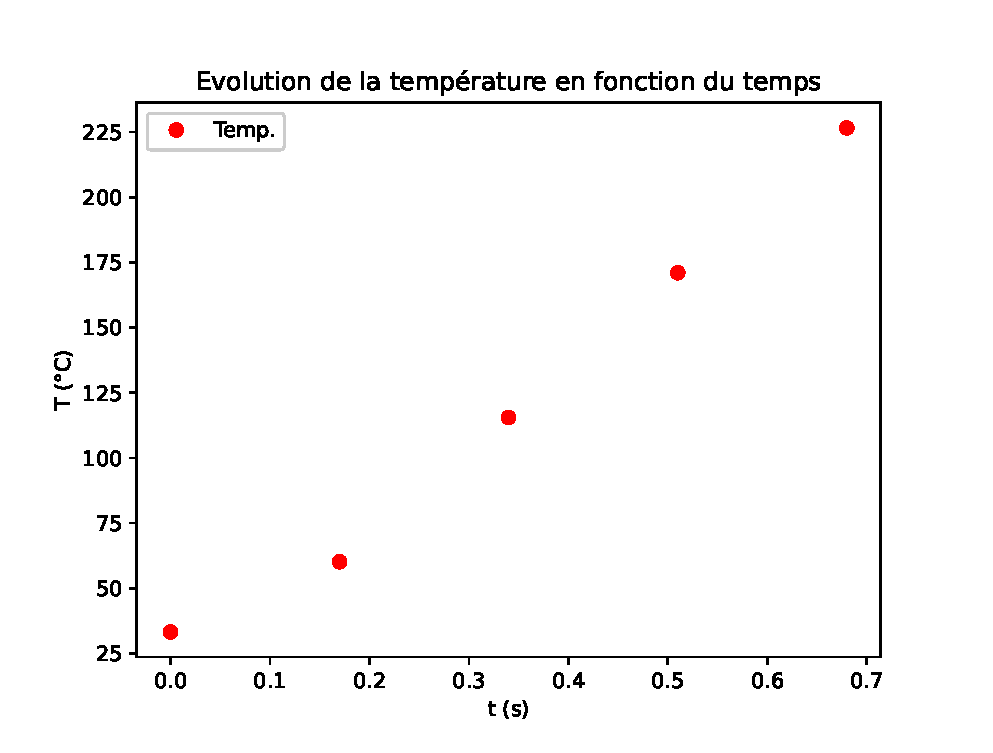
\includegraphics[width=0.6\textwidth]{image/Figure_1.eps}
\caption{Courbe à tracer}
\label{Figure_1}
\end{figure}

\vspace{5mm}
Il est également possible de tracer des histogrammes avec la commande \texttt{plt.hist} ou la commande \texttt{plt.bar}.

\vspace{5mm}
\Q{Tester et commenter les lignes de code suivantes :}
\begin{codePython}
import random as rd
import matplotlib.pyplot as plt
y=[]
for i in range(1,201):
    y.append((rd.randint(1,100)))
plt.figure()
plt.subplot(211)
plt.hist(y, 10, color='r')
plt.subplot(212)
plt.bar([i for i in range(200)], y, color=[0.2,0.5,0.8])
plt.show()
\end{codePython}

\newpage

\section{Exploiter les données enregistrées sur le système Comax}
Dans cette partie, on va s’appuyer sur un support de TP qui est utilisé aux oraux de concours : le système CoMax présenté sur la figure 1. Ce système est une adaptation pédagogique de la solution industrielle ZE de SAPELEM. Le principe de fonctionnement de ces deux systèmes repose sur l’utilisation d’un système de levage motorisé, associé à une poignée, équipée d'un capteur d’effort (voir Figure~\ref{sys_comax}).

\begin{figure}[!h]
\centering
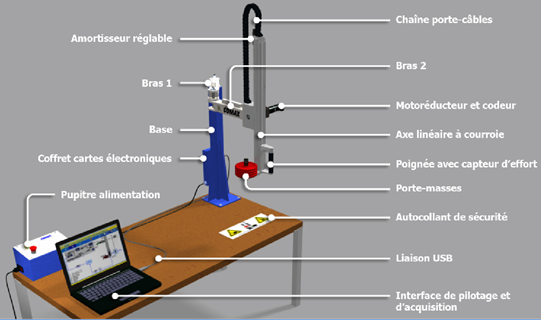
\includegraphics[width=0.8\textwidth]{image/sys_comax.png}
\caption{Présentation du système Comax}
\label{sys_comax}
\end{figure}

\subsection{Extraction des données expérimentales}
Nous allons dans cette partie utiliser les résultats d’expérimentions sur le robot CoMax. Ces résultats sont fournis dans le fichier \textit{CoMax.txt}. Ils correspondent à un fichier brut avec les points de mesures expérimentales. 


\vspace{5mm}
\Q{Après avoir observé la structure du fichier \textit{CoMax.txt}, proposer des instructions permettant d'extraire sous deux listes distinctes \texttt{temps} et \texttt{q\_exp} les instants de prise d'échantillonnage et les positions codeur correspondantes en tops (nombre de points). Ces deux listes seront converties en tableaux Numpy (\texttt{import numpy as np}), grâce à la commande \texttt{liste=np.array(liste)}.}

\vspace{5mm}
La position de l'axe linéaire $X(t)$ [en mm] est liée à la position du moteur $q_m$ [en tops] renvoyée par le codeur selon la formule suivante : $X = \dfrac{3,41.q_m}{1000}$ 

\vspace{5mm}
\Q{Générer alors un tableau des positions verticales de l'axe nommé \texttt{X\_exp}, qui a une condition initiale nulle sur la position.}

\vspace{5mm}
\Q{Tracer l'évolution des positions mesurées expérimentales en fonction du temps, avec des croix bleues (+). On légendera correctement les axes, et on indiquera une légende du type : "points mesurés"}

\subsection{Étude des performances attendues du système}
Dans un second temps, nous allons modéliser le comportement attendu système. La modélisation du système est faite en amont du système réel, lors de la phase de conception, mais elle est importante pour comprendre un système réel afin de proposer des modifications affectant les performances.

Les réponses attendues en vitesse V(t) et en position X(t) de l’axe linéaire sont représentées en Figure~\ref{lois_horaires} . Les caractéristiques de la loi en vitesse sont les suivantes :
\begin{itemize}
\item l’instant de début de mouvement : $t_0=0 s$ ;
\item la position initiale et la vitesse initiale : $X(0)=X_0=0 m$ et $V(0)=0 m/s$;
\item l’accélération : $A_{cmax}=2,83 m/s^2$ ;
\item la vitesse maximale : $V_{max}=0,68 m/s$.
\end{itemize}

\begin{figure}[!h]
\centering
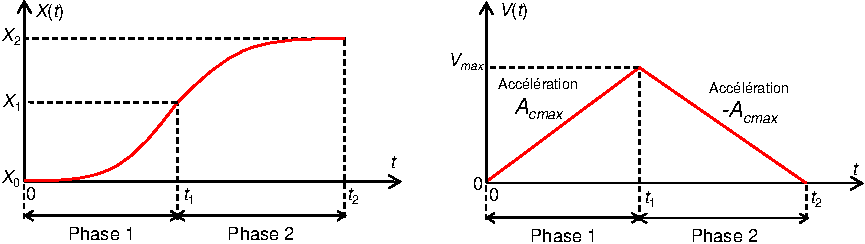
\includegraphics[width=0.9\textwidth]{image/lois_horaires.pdf}
\caption{Lois d'évolution en position (à gauche) et en vitesse (à droite) du CoMax}
\label{lois_horaires}
\end{figure}

On peut montrer par intégration successives, en tenant compte des conditions initiales que :

\vspace{0.5cm}
\begin{tabular}{|l|l|l|}
    \hline
     \textbf{Phase} &  \textbf{1} & \textbf{2}  \\
    \hline
     instant $t$  & $0\leq t <t_1$ & $t_1 \leq t \leq t_2$ \\
    \hline
     accélération $A(t)$  & $A_{cmax}$ & $-A_{cmax}$ \\
    \hline
     vitesse $V(t)$  & $A_{cmax}.t$ & $V_{max}-A_{cmax}.(t-t_1)$ \\
    \hline
     position $X(t)$  & $\dfrac{1}{2}.A_{cmax}.t^2$ & $X_1 + V_{max}.(t-t_1) - \dfrac{1}{2}.A_{cmax}.(t-t_1)^2$  \\
    \hline
\end{tabular}

On notera que : $X_1 = X(t_1)$, à l'issue de la phase 1 et $X_2=X(t_2)$, à l'issue de la phase 2.

\vspace{0.5cm}
\Q{Trouver les expressions littérales de $t_1$, $t_2$, $X_1$ et de $X_2$ en fonction de $A_{cmax}$ et de $V_{max}$.}

\vspace{0.5cm}
\Q{Concevoir deux fonctions \texttt{Loi\_Vitesse} et \texttt{Loi\_position} prenant en argument un instant $t$ et permettant de retourner la vitesse, respectivement la position, à cet instant. (A noter que l'on pourra introduire des variables globales, comme $t_1$, $t_2$, etc.)}

\vspace{0.5cm}
On rappelle que la commande \texttt{y = np.zeros(n)} permet de générer un tableau de taille $n \times 1$ contenant des 0.  

\vspace{0.5cm}
\Q{Construire deux tableaux \texttt{X\_th} et \texttt{V\_th} où sont stockées les positions théoriques commandées, respectivement vitesses théoriques aux instants définis dans le tableau \texttt{temps}. Superposer la courbe d'évolution de la position théorique sur les points expérimentaux, obtenus précédemment (tracé en vert, ligne continue, avec légende explicite). Sur une nouvelle figure tracer en vert, trait continu, l'évolution de la vitesse théorique}.


\subsection{Quantification et analyse des écarts}

Nous allons quantifier l’écart de performance entre l’exigence du cahier des charges et le système réel. Pour cela, nous allons calculer les écarts et utiliser des outils de statistique pour quantifier ces écarts.

On définit l'écart relatif en \% $\delta_\%$ entre une valeur théorique $x_{th}$ et une valeur expérimentale $x_{exp}$ : $\delta_\%=\displaystyle\left\lvert  \dfrac{x_{exp}-x_{th}}{x_{th}} \right\rvert$ 

\vspace{0.5cm}
\Q{Concevoir une fonction \texttt{Calcul\_ecarts} prenant en arguments deux tableaux à une dimension et retournant un tableau \texttt{Delta\_X} de même dimension où sont stockés les écarts relatifs entre chacune des valeurs des deux tableaux spécifiés en arguments d'entrée.}

\vspace{0.5cm}
\Q{Tracer un histogramme montrant l'évolution des écarts relatifs en position en fonction du numéro de la mesure (on utilisera \texttt{plt.bar} et \texttt{plt.subplot}). On n'évaluera pas l'écart relatif sur la première valeur (nulle).}

\vspace{0.5cm}
On rappelle ici quelques notions de statistiques :
\begin{itemize}
    \item La médiane d'un ensemble de valeurs (échantillon, population, distribution de probabilités) est une valeur qui partage la série en deux parties de même effectif.
    \item L’écart type est défini comme la moyenne quadratique des écarts par rapport à la moyenne. Il a la même dimension que la variable statistique étudiée.
\end{itemize}

\vspace{0.5cm}
\Q{Écrire une fonction \texttt{Calculs\_stats} permettant, à partir d'un tableau \texttt{T} passé en argument, de retourner un tuple de 3 valeurs : moyenne, médiane et écart type. \textit{Indication :} On pourra utiliser les fonctions de la bibliothèque numpy (\texttt{np.sum(T)}, pour faire la somme de tous les éléments du tableau \texttt{T}, \texttt{np.sort(T)}, pour trier le tableau \texttt{T} dans l'ordre croissant. Appliquer le résultat au tableau \texttt{Delta\_X}.}

\vspace{0.5cm}
\Q{Comparer les résultats en utilisant les fonctions suivantes : \texttt{np.mean}, pour la moyenne ; \texttt{np.median}, pour la médiane et \texttt{np.std}, pour l'écart type}
\label{LastPage}
\end{document}